\chapter{Main Window}
\label{cha:Main Window}
\section{Environment of the Main Window}

\begin{figure}[H]
    \centering
    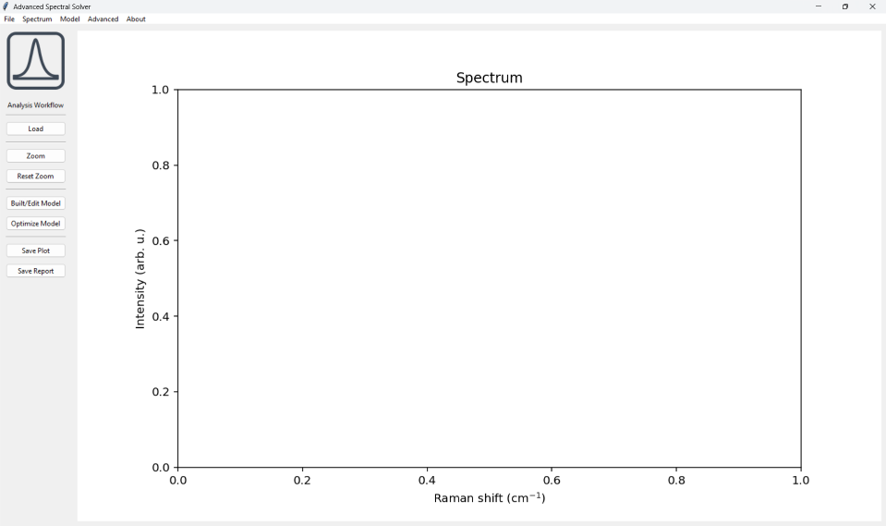
\includegraphics[width=1\linewidth]{Resources/ASS2_GUI.png}
    \caption{Graphical User Interface of the Advanced Spectral Solver}
    \label{GUI_main}
\end{figure}

The primary window of this application presents a straightforward and user-friendly workflow. Within the left panel (figure \ref{GUI_main}), there is a button sequence designed to guide you step by step through the essential analysis of the spectrum. These buttons are:

\begin{itemize}
    \item Load
    \item ZOOM
    \item Reset Zoom
    \item Build/Edit Model
    \item Optimize Model
    \item Save Plot
    \item Save Report
\end{itemize}

Each of these functions will be described separately.

Another method to access various functions, including the more advanced options, is through the top menu.

\section{Load - Import of Data}

This app is programmed to read \texttt{.txt} files exported from the HORIBA and WITec spectrometers. Since the structure of exported files can vary between instruments and measurement modes, import routines are designed to be flexible and adaptable.

To simplify the workflow for repeated analysis or data sharing, the app also supports its own lightweight \textbf{Default format}. This format contains no headers or metadata — just raw spectral data — making it easy to export a specific region of interest and re-import it later for further analysis. This approach enables users to focus on the parts of the spectrum that matter most, without the overhead of parsing complex file structures. Additionally, this format is readily interpretable by various software applications such as Excel, Origin, and similar programs.

\paragraph{Note:} The "User defined" format allows users to customize and define their own structure of data files. Formats like .txt, .csv, or Excel .xlsx files can be imported with definition separator, skip\_rows (to bypass file headers), usecols (to determine which columns are loaded), and file encoding ("ansi" and "utf-8" are the most common). These options can be individually configured through "File/Modify user spectrum details," where you can input your settings and save them using the "Apply" button.

\begin{figure}[H]
    \centering
    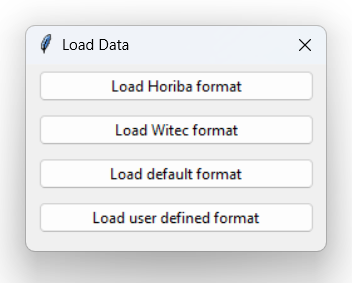
\includegraphics[width=0.35\linewidth]{Resources/Loader_window.png}
    \caption{Loader window with Horiba, Wited, Default, and User option}
    \label{loader_window}
\end{figure}

Activating the Load button will launch a window that prompts the user to choose the file type to be loaded (HORIBA, WITec, Default, or User defined, figure \ref{loader_window}). Upon selecting the file type, the user selects the desired file using a file browser. The import process for each file type can be accelerated by using shortcut keys that will open the file browser directly: 'Ctrl+h' for HORIBA, 'Ctrl+w' for WITec, 'Ctrl+d' for Default, and 'Ctrl+u' for User.

An equivalent outcome can be achieved via the "File" button in the top menu(figure \ref{GUI_main}). The only difference is that this way allows toggling the "User format definition" environment.

\section{ZOOM}
Clicking on a ZOOM button will trigger the span selector, enabling the user to choose a range along the Raman shift axis for analysis. Once activated, the user can select the region by holding down the left mouse button and dragging the cursor across the desired Raman shift spectrum. Following the release, the graph will automatically refresh along both the Raman shift axis, as determined by the span selector, and the intensity axis in accordance with the displayed data.
\par
If it is necessary to store data for future reference, you can right-click on the plot and choose the "Save spectrum" option. This action enables you to save the currently displayed segment of the spectrum as a text file in the "default format".
\section{Reset Zoom}
Clicking the "Reset Zoom" button will simply reset the boundaries set by the ZOOM span selector.
\section{Build/Edit model}
\label{model_building}
Pressing this button opens a new window where users can construct the composite model using predefined profile functions. A new function can be incorporated into the model with the "Add function" button. Subsequently, a new dropdown menu will appear on the right panel of the model builder window. After selecting a function, a function label and an input field for function parameters will be available. The GUI of the model builder can be seen in the figure \ref{model_builder}.

\begin{figure}[H]
    \centering
    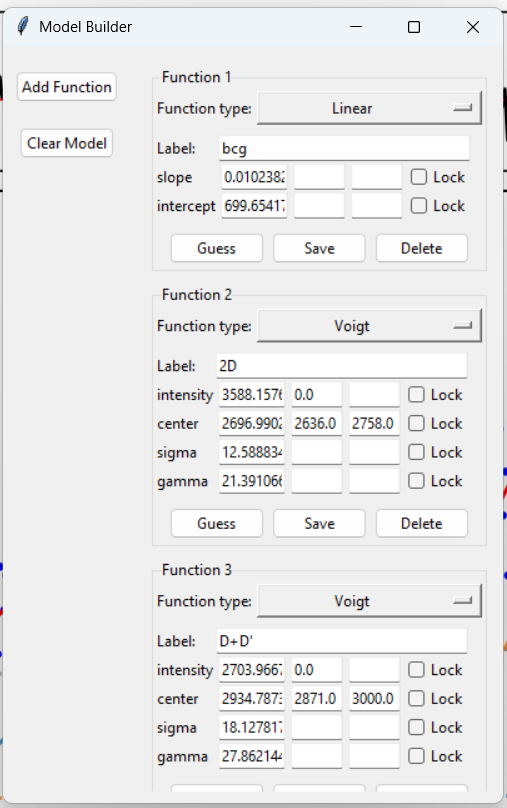
\includegraphics[width=0.5\linewidth]{Resources/model_builder.png}
    \caption{Model builder window with already defined functions}
    \label{model_builder}
\end{figure}

\par
While the label is optional, it helps to navigate the composite model, particularly in complex models. Labels support basic mathematical formatting using \texttt{matplotlib-style}-style syntax: use underscores for subscripts (e.g., \texttt{"G\_\{2D\}"} produces $G_\mathrm{2D}$), the circumflex sign (\textasciicircum) for superscripts (e.g., \texttt{"I\textasciicircum 2"} gives $I^2$), and prepend a backslash to insert Greek letters (e.g., \texttt{"\textbackslash alpha"} gives $\alpha$). When using the mathematical format whole label need to be closed between dollar signs, for example: \$random label\$. By default, the math formatted text is written in italics. if you want to have your label written in normal text, you need to add \textbackslash mathtm\{\} at the beginning of the label. All together label can look like \$\textbackslash mathrm\{\textbackslash Gamma\_\{2D\}\}\$ which will produce label $\mathrm{\Gamma_{2D}}$.
\par
The first column for parameter entry is for the parameter value, with the next two columns specifying the lower and upper boundaries, preventing the parameter from surpassing these limits during fitting. Users can input these boundaries manually or opt for the "Guess" feature, selecting the spectral region to be described by the chosen profile function with the span selector. Peak parameter estimation is based on the residual spectrum (raw spectrum minus the defined model), making it crucial to define the background function as an initial step in model building. Following selection, the function values and some boundaries are automatically populated. The peak intensity's lower boundary is set at 0 to avoid fitting negative peaks, and the peak position's boundaries are confined within the selection limits, preventing the peak from shifting outside its designated area. If the estimation is imprecise or requires adjustment, all parameters can be manually modified. It \textbf{is} important to note that a function won't appear in the composite model until it is saved using the save button. 
\par
When the app hosts an active composite model, it automatically displays the residual spectrum in the upper panel of the app's graph area, while the main plot showcases the raw data alongside the composite model and all individual functions (like in the figure \ref{multipeak_fit}). All peak functions are charted against the secondary right axis, with the left axis reserved for raw data, the composite model, and background functions (Linear and Sigmoid at present). To eliminate the function from the composite model, you just need to press the "Delete" button.

\begin{figure}[H]
    \centering
    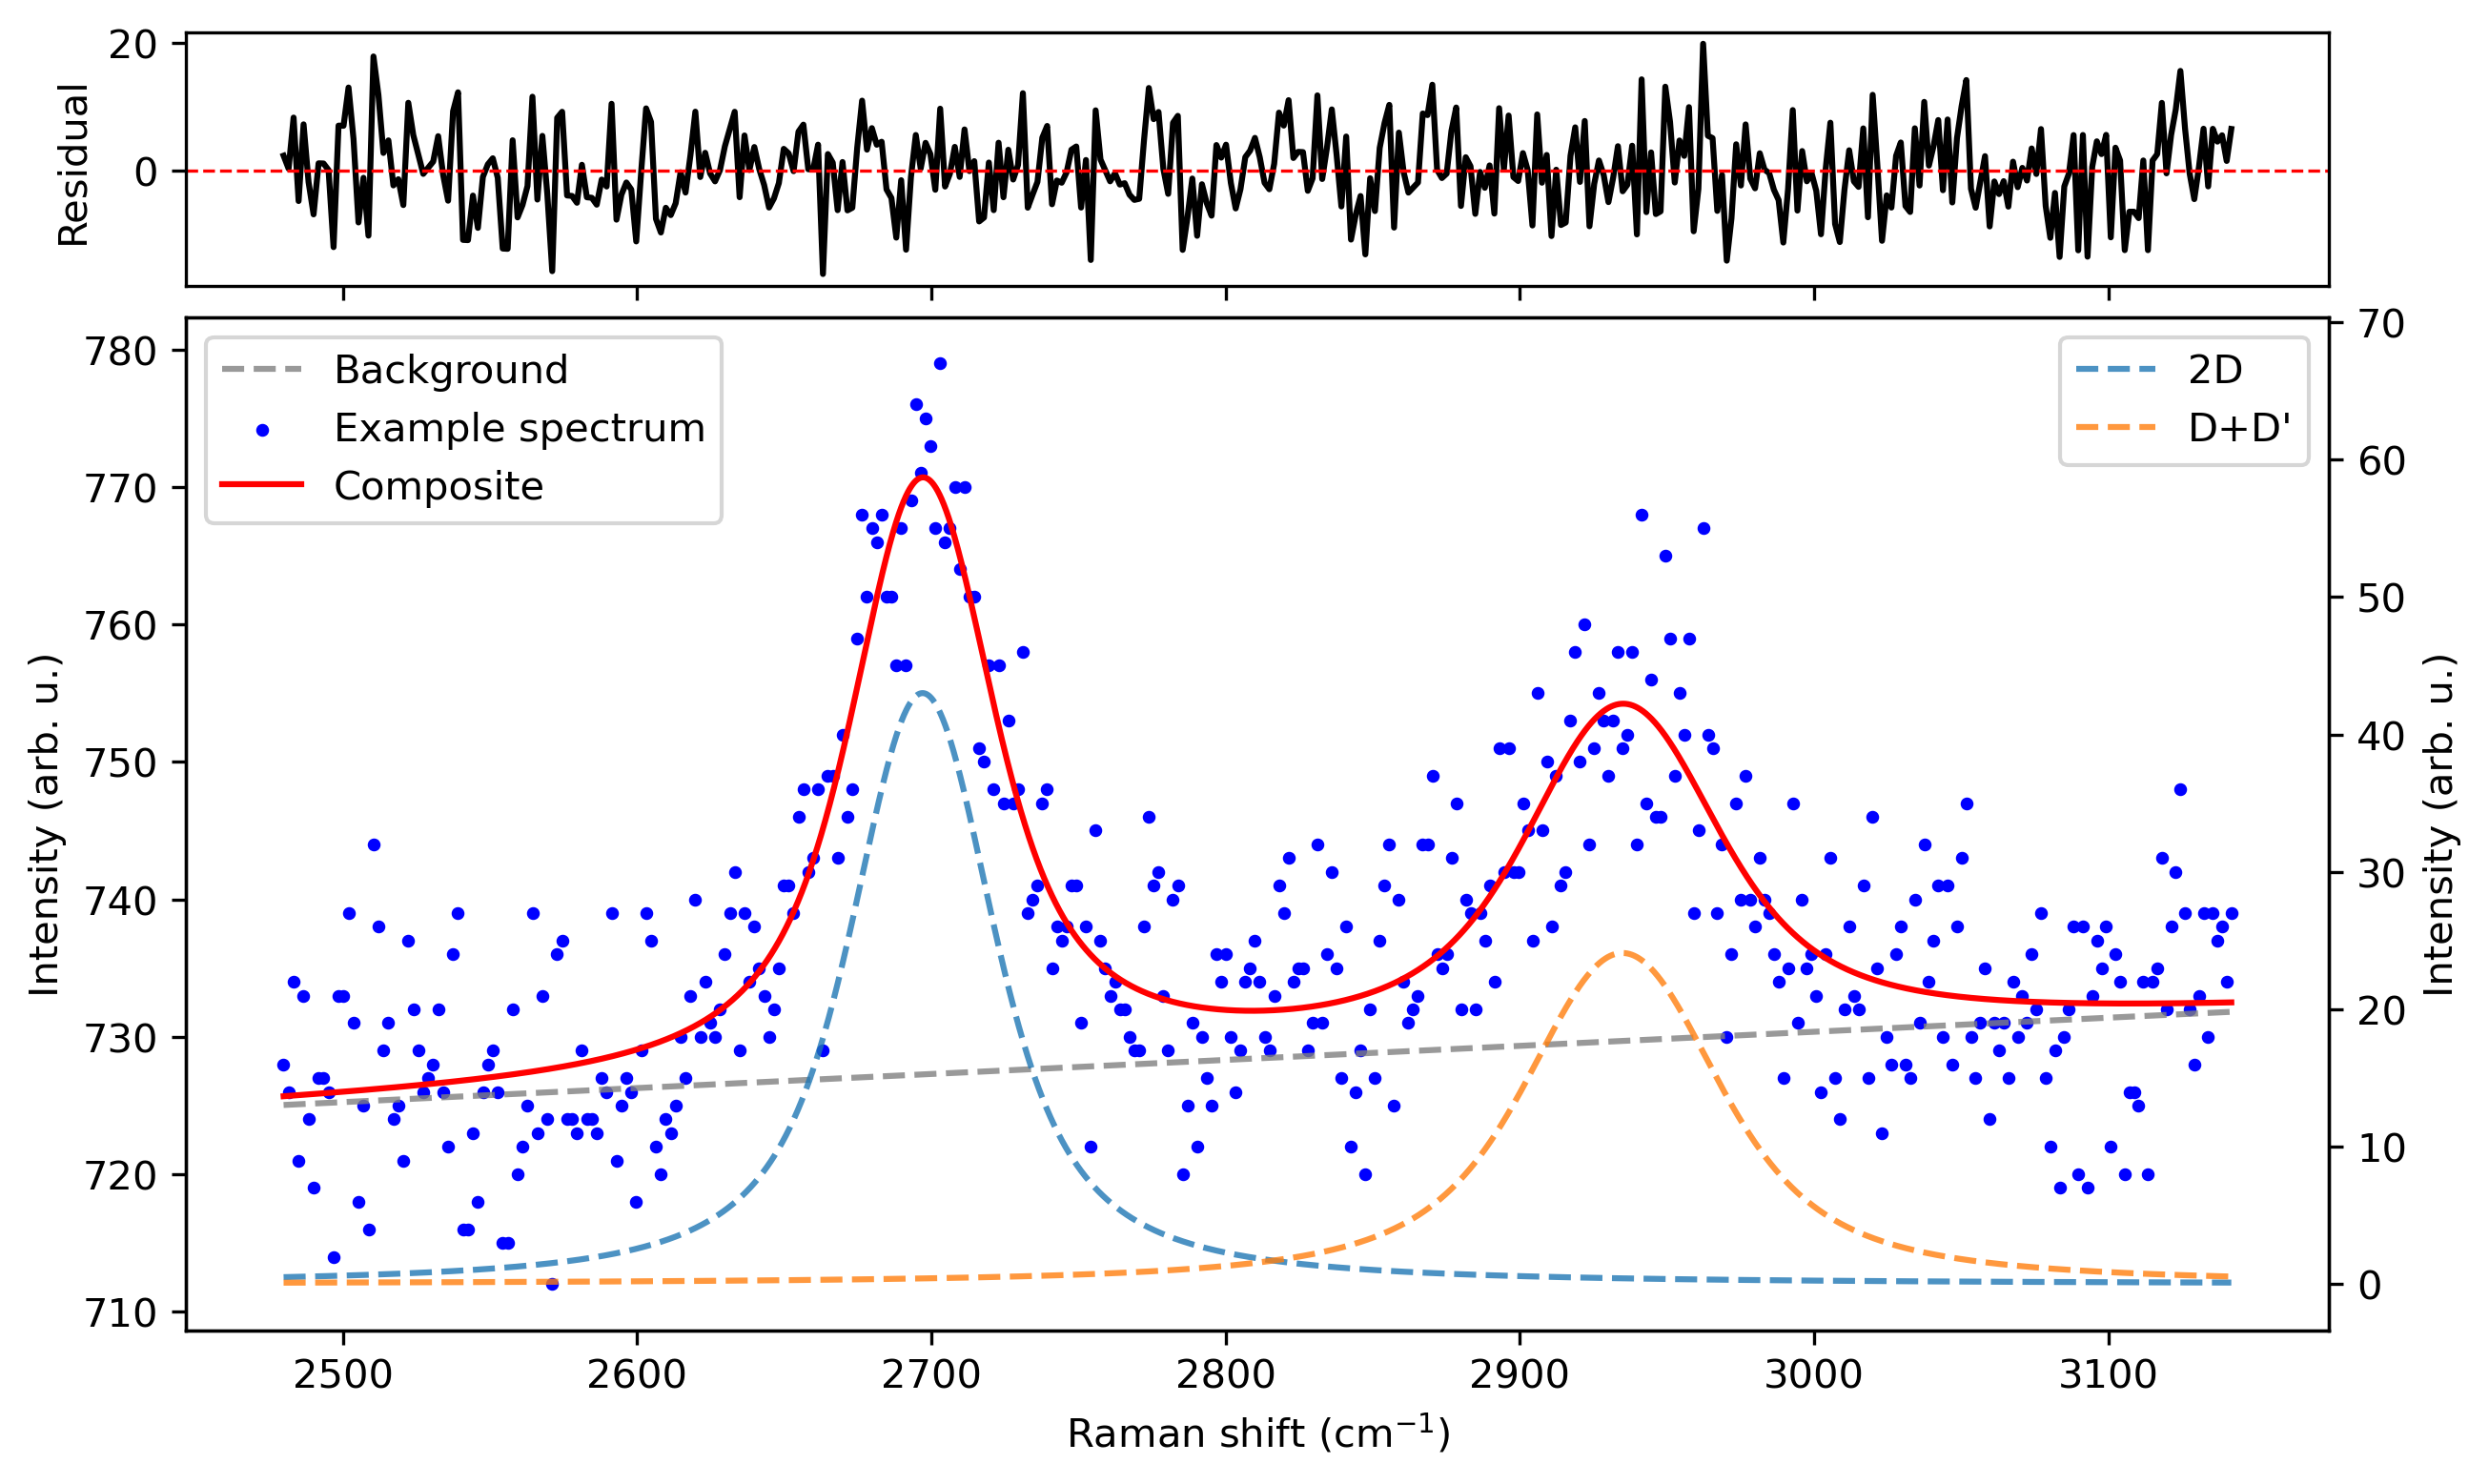
\includegraphics[width=0.75\linewidth]{Resources/multipeak_fit.png}
    \caption{Multipeak fit of the defective graphene sample in region of 2D and D+D' band.}
    \label{multipeak_fit}
\end{figure}
\par
The function that has been defined can be saved and retrieved as a .json file. This capability provides an opportunity to reuse models that were previously created, which is particularly useful when conducting analyses on similar datasets. Users can save and access the model through the menu at the top, under the "Model" section.
\par
If a user needs to remove the entire model, for instance, to analyze a different spectral region or a separate dataset, the "Clear model" option will delete all functions defined in the "Model builder window".
\par
A list of the available functions with explanations of their parameters can be find below:
\subsection{Lorentzian}
The Lorentzian function models peaks with long tails, typical of lifetime broadening:

\begin{equation}
L(x) = \frac{I}{\pi \cdot \Gamma \left[1 + \left(\frac{x - x_0}{\Gamma}\right)^2 \right]}
\end{equation}

\textbf{Parameters:}
\begin{itemize}
    \item $I$ – Integrated intensity (area under the curve)
    \item $x_0$ – Peak center
    \item $\mathrm{FWHM} = 2\Gamma$ – Full width at half maximum
\end{itemize}

\subsection{Gaussian}
The Gaussian function is ideal for symmetric peaks influenced by noise or instrument resolution:

\begin{equation}
G(x) = \frac{I}{\sigma \sqrt{2\pi}} \exp\left(-\frac{(x - x_0)^2}{2\sigma^2}\right)
\end{equation}

\textbf{Parameters:}
\begin{itemize}
\item $I$ – Total area under the curve
\item $x_0$ – Peak center (mean)
\item $\mathrm{FWHM} = 2\sqrt{2 \ln 2} \cdot \sigma$
\end{itemize}

\subsection{Voigt}
The Voigt profile is a convolution of Gaussian and Lorentzian broadening:

\begin{equation}
V(x) = I \cdot \mathrm{Voigt}(x - x_0, \sigma, \gamma)
\end{equation}

\textbf{Parameters:}
\begin{itemize}
\item $I$ – Area under the peak
\item $x_0$ – Peak center
\item $\sigma$ – Standard deviation (Gaussian part)
\item $\gamma$ – Half-width at half-maximum (Lorentzian part)
\end{itemize}

\subsection{Asymmetrical Lorentzian}
This variation introduces asymmetry to the Lorentzian profile:

\begin{equation}
AL(x) = \frac{I}{\pi \cdot \Gamma(x) \left[1 + \left(\frac{x - x_0}{\Gamma(x)}\right)^2 \right]}, \quad \Gamma(x) = \frac{\mathrm{FWHM}}{2} (1 + \alpha(x - x_0))
\end{equation}

\textbf{Parameters:}
\begin{itemize}
\item $I$ – Integrated intensity
\item $x_0$ – Peak center
\item $\mathrm{FWHM}$ – Full width at half maximum for symmetric case
\item $\alpha$ – Asymmetry parameter ($\alpha = 0$ gives symmetric Lorentzian)
\end{itemize}

\subsection{Fano Resonance}
The Fano function describes an asymmetric resonance due to quantum interference:

\begin{equation}
F(x) = I \cdot \frac{(q + \epsilon)^2}{1 + \epsilon^2}, \quad \epsilon = \frac{x - x_0}{\Gamma}
\end{equation}

\textbf{Parameters:}
\begin{itemize}
\item $I$ – Area under the resonance
\item $x_0$ – Resonance position
\item $\mathrm{FWHM} = 2\Gamma$ – Width of the resonance
\item $q$ – Asymmetry parameter
\end{itemize}

\subsection{Linear}
Simple linear trend used for baseline correction:

\begin{equation}
y(x) = m \cdot x + b
\end{equation}

\textbf{Parameters:}
\begin{itemize}
\item $m$ – Slope
\item $b$ – Intercept
\end{itemize}

\subsection{Sigmoid}
Smooth transition often used for step-like backgrounds:

\begin{equation}
S(x) = \frac{A}{1 + e^{-(x - x_0)/s}} + B
\end{equation}

\textbf{Parameters:}
\begin{itemize}
\item $A$ – Amplitude of the step
\item $x_0$ – Center of the transition
\item $s$ – Steepness (lower = sharper)
\item $B$ – Baseline offset
\end{itemize}

\section{Optimize model}
Once the model is defined, you can start the fitting process by clicking the "Optimize" button. This will trigger an optimization procedure that minimizes the sum of squared residuals using a non-linear approach. This is accomplished with the SciPy (scientific Python library) function \texttt{curve\_fit}, and additional information is available in the official documentation.
\par
After finalizing the fit, users are presented with multiple methods to save the results. These can be accessed by right-clicking on the graph.
\begin{itemize}
    \item Save plot - saves the visual representation as a .png file
    \item Save report - generates a .txt file containing the optimized parameters and fitting statistics, which will be explained in detail later
    \item Save both - concurrently stores both the Plot and Report in the chosen directory
    \item Save data - exports an Excel file containing the raw data shown, the composite model, and each individual function
    \item Save spectrum - save the currently displayed spectrum in a default format (no header, just two columns of data) for possible later use
\end{itemize}

\subsection{Structure of the report file}
The report file contains the values of the optimized parameters, including their errors from the fit.
To help evaluate the quality and reliability of the fitted model, the application also computes several statistical metrics based on the residuals between the data and the model. These include $R^2$, adjusted $R^2$, RMSE, AIC, and BIC. Also, the covariance and correlation matrices are included.
\par
\subsubsection*{Parameter Errors (Uncertainties)}

Each fitted parameter is reported with a corresponding standard error, which reflects the uncertainty in its value based on the local curvature of the cost function. Smaller errors indicate higher confidence in the parameter estimate.

\subsubsection*{Coefficient of Determination ($R^2$)}
\[
R^2 = 1 - \frac{\mathrm{SS}_{\mathrm{res}}}{\mathrm{SS}_{\mathrm{tot}}}
\]
\begin{itemize}
    \item $\mathrm{SS}_{\mathrm{res}} = \sum (y_i - f_i)^2$: residual sum of squares.
    \item $\mathrm{SS}_{\mathrm{tot}} = \sum (y_i - \bar{y})^2$: total variance of the data.
\end{itemize}

$R^2$ indicates how well the model explains the variance in the data. A value close to 1 suggests a good fit.

\subsubsection*{Adjusted $R^2$}
\[
R^2_{\mathrm{adj}} = 1 - (1 - R^2) \cdot \frac{n - 1}{n - p}
\]
\begin{itemize}
    \item $n$ – Number of data points
    \item $p$ – Number of fitted parameters
\end{itemize}

Unlike $R^2$, the adjusted $R^2$ accounts for the complexity of the model. It penalizes the use of unnecessary parameters and is better suited for comparing models with different numbers of variables.

\subsubsection*{Root Mean Square Error (RMSE)}
\[
\mathrm{RMSE} = \sqrt{ \frac{1}{n} \sum (y_i - f_i)^2 }
\]

RMSE gives an absolute measure of the average deviation between the data and the model. Lower values indicate a better fit.

\subsubsection*{Akaike Information Criterion (AIC)}
\[
\mathrm{AIC} = n \cdot \ln\left(\frac{\mathrm{SS}_{\mathrm{res}}}{n}\right) + 2p
\]

AIC evaluates model quality by balancing goodness of fit and complexity. Lower AIC values indicate a more parsimonious (efficient) model. Useful for comparing different model structures.

\subsubsection*{Bayesian Information Criterion (BIC)}

\[
\mathrm{BIC} = n \cdot \ln\left(\frac{\mathrm{SS}_{\mathrm{res}}}{n}\right) + p \cdot \ln(n)
\]

BIC serves a similar purpose to AIC but penalizes model complexity more heavily. Particularly useful when the goal is to identify the simplest adequate model.
\paragraph{Note:} AIC and BIC are only meaningful when comparing fits on the same dataset. They are not absolute indicators of fit quality, but they help guide model selection.

\subsubsection*{Covariance Matrix}

The covariance matrix describes how the uncertainties of different parameters are interrelated. For parameters $a_i$ and $a_j$, the covariance $\mathrm{Cov}(a_i, a_j)$ measures how variations in one parameter correspond to variations in the other.

\begin{itemize}
    \item \textbf{Diagonal elements:} Variances of each parameter, i.e., $\mathrm{Var}(a_i) = \sigma_i^2$.
    \item \textbf{Off-diagonal elements:} Covariances between pairs of parameters.
\end{itemize}

Large off-diagonal values suggest that the corresponding parameters are not independently determined; a change in one may be partially compensated by a change in another.

\subsubsection*{Correlation Matrix}

The correlation matrix is a normalized version of the covariance matrix. Each element is calculated as:

\[
\mathrm{Corr}(a_i, a_j) = \frac{\mathrm{Cov}(a_i, a_j)}{\sigma_i \, \sigma_j}
\]

where $\sigma_i$ and $\sigma_j$ are the standard errors of parameters $a_i$ and $a_j$.

\begin{itemize}
    \item Values range from $-1$ to $+1$.
    \item $\mathrm{Corr}(a_i, a_j) = 0$ indicates statistical independence.
    \item Values close to $\pm1$ indicate a strong linear dependence between the parameters.
\end{itemize}

\paragraph{Note:} Strong correlations (e.g., $|\mathrm{Corr}| > 0.95$) may indicate that the model is over parameterized or that the parameters are physically redundant.

\section{Save plot}
This button will save currently rendered graphics; everything that the app displays on the main canvas will be saved as a .png picture. This option is also accessible by right-clicking on the canvas and selecting the particular function.
\section{Save report}
This button will save just the report of the fit in .txt format. This option is also accessible by right-clicking on the canvas and selecting the particular function.